\glsresetall
A sensible first case study for \gls{qmla} is to search within a closed space of models
    targeting some typical quantum systems; 
    in particular we consider Ising, Heisenberg and Hubbard formalisms as a test-bed for the \gls{qmla} framework. 
We can prescribe a set of models for \gls{qmla} to consider, $\mathbb{H}$,
    from which it will choose a \gls{champion model}, $\hp$.
By including the \gls{true model}, $\ho \in \mathbb{H}$, 
    then \gls{qmla} should perform well at retrieiving $\hp=\ho$,
    provided its core assumptions are reliable, 
    i.e. that model training, comparison and selection are 
    feasible on meaningful models.
\par 

This application can be useful, for example, for expedited device calibration:
    suppose we wish to characterise a new, \emph{untrustued} quantum simulator/device, $S_u$, 
    and we have access to a \emph{trusted}\footnotemark \  simulator, $S_t$. 
In order to perform this calibration, 
    we treat $S_u$ as the system, \gls{q}, i.e. we call upon it to retrieve the datum $d$ in \cref{eqn:likelihood}, 
    where the calculation of the \glspl{likelihood}  for each \gls{particle} are computed through $S_t$. 
If $S_u$ is reliable, the data from its calculations will be consistent with some $\ho$ of our choosing. 
Conversely, miscalibrations will mainfest as imperfectly implemented gates/steps in the calculation of the system's likelihood, 
    and so would result in data inconsistent with $\ho$. 
Therefore, if we can prescribe the most likely miscalibrations, it may be feasible to compose a set 
    of models, $\mathbb{H}$, which represent those cases, and search for $\hp$ only within $\mathbb{H}$,
    to identify the dominant error mechanism(s). 
For example, by encoding in $\ho$ the connections between every pair of qubits on the device qubits,
    we can compose candidate models of restricted connectivity, for instance where some pairs of qubits are disconnected, 
    and hence discover whether the device allows arbitrary two-qubit gates, 
    and which pairs are disallowed. 
\footnotetext{Note: here a classical computer can fulfil the role of the trusted simulator.}
\par

In this chapter we perform such a study of the \gls{qmla} framework itself, 
    by manually defining target and candidate models in simulation, 
    given by lattice structures.
We test the protocol by varying the physical systems it aims to represent, 
    and finish by demonstrating that \gls{qmla} can classify the family of models 
    underlying the target system, when allowed explore several families.  

\section{Lattices}\label{sec:lattices}
In each case examined in this chapter, \gls{qmla} will aim to identify the \gls{true model}, $\ho$, 
    determined by a series of target systems, \gls{q}.
\gls{q} represents some physical configuration; we specify the configuration of 
    all models through unique \emph{lattices}. 
The goal of \gls{qmla} is then to identify the structure of the true lattice,
% We first consider \gls{q} as some lattice, where \gls{qmla} attempts to identify the structure of the lattice. 
    while the set of viable models are specified by alternative lattices.
Due to simluation constraints, because we train models through exact unitary evolution, 
    we are restricted to $\sim8$-qubit \glspl{hamiltonian}, so we only consider lattices which can 
    be simulated in this limit. 
The \gls{es} in this chapter is then simply to propose a set of models with no further model generation, 
    with comparisons between all pairs of models through \glspl{bf}.
\par

Connectivity between lattice sites is achieved within the specific \gls{hamiltonian} formalisms
    introduced in the following sections, 
    although in general we write $\mathcal{C} = \{\bkl \}$ as the set of connected pairs $\bkl$, 
    such that the \gls{hamiltonian} for a given lattice can be thought of as 
    some function of its configuration, $\hat{H}\bk{\al, \mathcal{C}}$, 
    where $\al$ is the usual vector of multiplicative parameters corresponding to each term in the Hamiltonian.
Then, we can specify candidate models only by their $\mathcal{C}$, 
    e.g. a 3-site chain can be summarised by $\mathcal{C}= \{ \langle 1,2 \rangle, \langle 2,3 \rangle\}$, 
    whereas a fully connected 3-site lattice (i.e. a triangle) is given by 
    $\mathcal{C}= \{ \langle 1, 2 \rangle, \langle 1, 3 \rangle, \langle 2, 3 \rangle\}$. 
We can then summarise the set of candidate models through the descriptions of lattice configurations, 
    corresponding to those depicted in \cref{fig:lattices}:
\begin{easylist}[enumerate]
    \ListProperties(Numbers=l)
    & 2-site chain
    & 3-site chain
    & 3-site fully connected (triangle)
    & 4-site fully conneted (square)
    & 4-site linearly connected (loop)

    & 4-site chain
    & 5-site chain
    & 6-site chain
    & 5-site fully connected (pentagon)
    & 6-site partially connected (grid)
\end{easylist}


\begin{figure}
    \begin{center}
        \begin{subfigure}{2.25cm}
            \begin{center}
                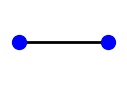
\includegraphics{theoretical_study/figures/lattices/_2_site_chain.jpg}                        
            \end{center}
            \caption{}
        \end{subfigure}
        \qquad
        \begin{subfigure}{2.25cm} 
            \begin{center}
                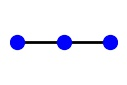
\includegraphics{theoretical_study/figures/lattices/_3_site_chain.jpg}
            \end{center}
            \caption{}
        \end{subfigure}
        \qquad
        \begin{subfigure}{2.25cm} 
            \begin{center}
                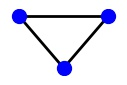
\includegraphics{theoretical_study/figures/lattices/_3_site_lattice_fully_connected.jpg}        
            \end{center}
            \caption{}
        \end{subfigure}
        \qquad
        \begin{subfigure}{2.25cm} 
            \begin{center}
                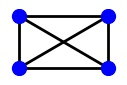
\includegraphics{theoretical_study/figures/lattices/_4_site_lattice_fully_connected.jpg}        
            \end{center}
            \caption{}
        \end{subfigure}
        \qquad
        \begin{subfigure}{2.25cm} 
            \begin{center}
                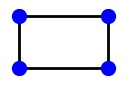
\includegraphics{theoretical_study/figures/lattices/_4_site_square.jpg}        
            \end{center}
            \caption{}
        \end{subfigure}
        \\
        \begin{subfigure}{2.25cm} 
            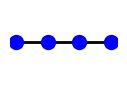
\includegraphics{theoretical_study/figures/lattices/_4_site_chain.jpg}        
            \caption{}
        \end{subfigure}
        \qquad
        \begin{subfigure}{2.25cm} 
            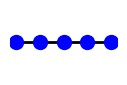
\includegraphics{theoretical_study/figures/lattices/_5_site_chain.jpg}        
            \caption{}
        \end{subfigure}
        \qquad
        \begin{subfigure}{2.25cm} 
            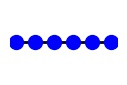
\includegraphics{theoretical_study/figures/lattices/_6_site_chain.jpg}        
            \caption{}
        \end{subfigure}
        \qquad
        \begin{subfigure}{2.25cm} 
            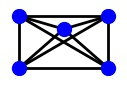
\includegraphics{theoretical_study/figures/lattices/_5_site_lattice_fully_connected.jpg}        
            \caption{}
        \end{subfigure}
        \qquad
        \begin{subfigure}{2cm} 
            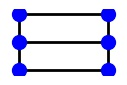
\includegraphics{theoretical_study/figures/lattices/_6_site_grid.jpg}        
            \caption{}
        \end{subfigure}
    \end{center}
    \caption[Lattices for prescribed QMLA exploration strategy]{
        Lattices used for prescribed models test for \gls{qmla}.
        Lattices are characterised by the connectivity of their sites; 
            dotted lines show connection between pairs of sites.                 
    }
    \label{fig:lattices}
\end{figure}

We will use this set of lattice configurations throughout the remainder of this chapter. 

\section{Ising model}\label{sec:ising}
The quantum Ising model -- otherwise known as the transverse field Ising model, hereafter simply the Ising model -- 
    is one of the most studied concepts in all of physics, 
    representing electrons on a lattice of $N$ sites, 
    where each electron can have \emph{spin} up or down 
    \cite{ising1925beitrag, onsager1944crystal, brush1967history}.
Interactions\footnotemark \ between spins $\bkl$ have strength $J_{kl}$, 
    and the transverse magnetic field acts on spin $k$ with strength $h_k$. 
The Ising model is usually stated as 
\begin{equation}
    \label{eqn:ising_standard_form}
    \hat{H}_I(\cc) = \sum_{\bkl \in \mathcal{C}} J_{kl}  \ \hat{\sigma}_k^z \ \hat{\sigma}_{l}^z + \sum_{k=1}^{N} h_k \hat{\sigma}_{k}^x.
\end{equation}
\footnotetext{
    The Ising model usually considers only nearest neighbour interaction. 
    Here we present the more general $\bkl$ which can connect any pair of sites, 
    and specify pairs in the set $\mathcal{C}$. 
}

The interaction term\footnotemark \ indicates the class of magnetism of the pair's interaction, i.e. 
\begin{equation}
    \label{eqn:ising_magnetism_cases}
    \begin{cases}
        J_{kl} < 0, \ \ \textrm{ferromagnetic}; \\
        J_{kl} > 0, \ \ \textrm{antiferromagnetic}; \\
        J_{kl} = 0, \ \ \textrm{noninteracting}.
    \end{cases}
\end{equation}
If all interaction pairs are described by the same case in \cref{eqn:ising_magnetism_cases}, 
    the entire system can be said belong to that class of magnetism. 

\footnotetext{
    Note: the terms $J_{kl}$ is often presented as $-J_{kl}$ in \cref{eqn:ising_standard_form}, 
        such that $J_{kl} > 0$ indicates ferromagnetism.
    Here we keep the parameter general, and set the sign implicitly when defining and learning the parameter, 
        so $J_{kl}>0$ corresponds to ferromagnetism. 
    This is a matter of convention and does not impact any of the further discussion. 
}

\par 
\subsection{Note on optimising the Ising model}\label{sec:ising_optimisation}
Many treatments of the Ising model seek to find the ground state
    of the system by optimising the configuration of spins in the system. 
This involves treating the Ising model classically, 
    effectively by neglecting the transverse magnetic field term $(h_k \rightarrow 0)$,
    such that the ground state is found by minimising the energy function
\begin{equation}
    \label{eqn:ising_energy_function}
    E_I = \braket{\psi | H_I | \psi} = 
    \sum_{\bkl \in \mathcal{C}} J_{kl}  \ \braket{ \psi |  \hat{\sigma}_k^z \ \hat{\sigma}_{l}^z | \psi }, 
\end{equation}
    where $\ket{\psi} = \ket{\psi_1} \otimes \ket{\psi_2} \dots \otimes \ket{\psi_N}$. 

This optimisation relies on the relationship between the Ising model with its eigenvalues and eigenstates:
    \cref{eqn:ising_energy_function} consists only of $\sz$ terms, and we have that 
\begin{equation}
    \sz \ket{+} = +1 \ket{+} \ \ \ ; \ \ \ 
    \sz \ket{-} = -1 \ket{-}. 
\end{equation}

Then, for a single pair of spins $\bkl$, we have
\begin{equation}
    \label{eqn:ising_spin_cases}
    \begin{split}
        \bra{+_{k} \ +_{l} } \hat{\sigma}^{z}_{k} \ \hat{\sigma}^z_{l}  \ket{+_{k} \ +_{l} } =  \bra{+_{k} \ +_{l} } (+1)(+1) \ket{+_{k} \ +_{l} } = +1, \\
        \bra{+_{k} \ -_{l} } \hat{\sigma}^{z}_{k} \ \hat{\sigma}^z_{l} \ket{+_{k} \ -_{l} } = \bra{+_{k} \ -_{l} } (+1)(-1) \ket{+_{k} \ -_{l} } = -1 , \\
        \bra{-_{k} \ +_{l} } \hat{\sigma}^{z}_{k} \ \hat{\sigma}^z_{l} \ket{-_{k} \ +_{l} } = \bra{-_{k} \ +_{l} } (-1)(+1) \ket{-_{k} \ +_{l} } = -1, \\
        \bra{-_{k} \ -_{l} } \hat{\sigma}^{z}_{k} \ \hat{\sigma}^z_{l} \ket{-_{k} \ -_{l} } = \bra{-_{k} \ +_{l} } (-1)(1) \ket{-_{k} \ -_{l} } = +1. \\
    \end{split}
\end{equation}
So, by restricting the individual spins to $\ket{\psi_k} \in \{\ket{+}, \ket{-}\}$, 
    we can equivalently consider every spin $s_k$ in the system
    as a binary variable $s_k \in \{\pm 1\}$,
    i.e. $s_k s_l = \pm 1$ in \cref{eqn:ising_spin_cases},
    such that the energy function
\begin{equation}
    \label{eqn:ising_energy}
    E_I(\mathcal{S}) = \braket{ \psi | \hat{H}_I | \psi } = \sum\limits_{\bkl \in \cc} J_{kl} \ \ s_k s_l
\end{equation}
    can be minimised by optimising the configuration $\mathcal{S} = s_1, \dots, s_N$, when the interaction terms $\{J_{\bkl}\}$ are known.
The optimal configuration $\mathcal{S}_0$ can then be mapped to a 
    state vector $\ket{\psi_0}$, i.e. the ground state of the system. 
\par 

While this task can be greatly simplified by the reduction in \cref{eqn:ising_spin_cases}, 
    meaning we do not have to compute any unitary evolution to evaluate \cref{eqn:ising_energy},
    it is still an expensive optimisation, because effectively it is a search over $\{ \ket{\psi }\}$, 
    so the search space has $2^N$ candidates \cite{onsager1944crystal, barahona1982computational}. 
This allows for a straightforward mapping between ground state search 
    and solving combinatorial optimsiation algorithms, namely \ttt{MAX-CUT}, 
    known to be NP-complete \cite{garey1979computers}, 
    allowing for proposed advantage in mapping computationally challenging problems to quantum hardware \cite{lucas2014ising}. 
This mapping underlies ongoing research into quantum annealing as a computational platform capable of providing 
    advantage for a specific family of problems \cite{santoro2006optimization, bapst2013quantum, johnson2011quantum}. 
\par

Crucially, our goal is \emph{not} to find the ground state of \gls{q}, 
    but instead to find the generator of its dynamics.
Therefore, we treat the Ising \emph{quantum mechanically}:
    instead of treating \cref{eqn:ising_standard_form} as the underlying mechanism for a cost function 
    to be optimised, i.e. \cref{eqn:ising_energy}, 
    we use quantum operators and do not necessarily restrict the \gls{probe} state $\ket{\psi}$, 
    allowing us to use \cref{eqn:ising_standard_form} within the \gls{likelihood} function \cref{eqn:likelihood}.

\subsection{Ising model cases}

We consider two cases: 
    firstly, where it is assumed that the strength of interactions $J_{k,l}$ are uniform (given by $J$);
    and secondly, where each interaction is assigned a unique parameter ($J_{kl}$).
In the first case, we can represent the Ising model for a given lattice configuration $\cc$ as 
\begin{equation}
    \label{eqn:ising_model_full}
    \hat{H}(\mathcal{C}) = 
        J \sum\limits_{\bkl \in \mathcal{C}} \s^{z}_{k} \s_{l}^{z} 
        + h \sum\limits_{k=1}^{N} \s^{x}_{k}, 
\end{equation}    
    allowing for the compact representation, following \cref{sec:models},
\begin{subequations}
    \label{eqn:ising_terms}
    \begin{equation}
        \vec{\alpha}_{I} = \irow{ J & h }
    \end{equation}
    \begin{equation}
        \terms_I = \icol{ 
            \sum\limits_{\bkl \in \mathcal{C}} \s^{z}_{k} \s_{l}^{z} \\
            \sum\limits_{k=1}^{N} \s^{x}_{k}
        }. 
    \end{equation}
\end{subequations}

In the more general second case, termed the \emph{fully parameterised} Ising model, we instead have the parameter and term sets

\begin{subequations}
    \label{eqn:ising_fully_parameterised}
    \begin{equation}
        \alpha_{I} = \{ J_{k,l}, \ h_k \}_{\bkl \in \cc}
    \end{equation}
    \begin{equation}
        \termset_I = \left\{ 
            \s^{z}_{k} \s_{l}^{z}, \ \
            \s^{x}_{k}
        \right\}_{\bkl \in \cc}. 
    \end{equation}        
\end{subequations}
    with unique parameters $J_{kl}$ associated with each interaction term $\s_k^z \s_l^z$, 
    and $h_k$ associated with each field term, $\s_k$. 
We summarise these cases in \cref{table:ising_models}.

\begin{table}[H]
    \begin{center}
        \begin{tabular}{crr}
             & $J_{\bkl}$  & $h_{k}$ \\
            \hline
            Standard & $J$ & $h$ \\
            Fully parameterised & $J_{\bkl}$ & $h_{k}$
        \end{tabular}
    \end{center}
    \caption[Forms of Ising model]{Forms of Ising model. Varying whether parameters $J_{\bkl}, h_k$ are shared 
        across terms result in distinct models. 
    }
    \label{table:ising_models}
\end{table}

\par 

\begin{figure}[t]
    \begin{center}
        % \QMLAfig{Nov_18/13_56/standard_ising_qhl.pdf}
        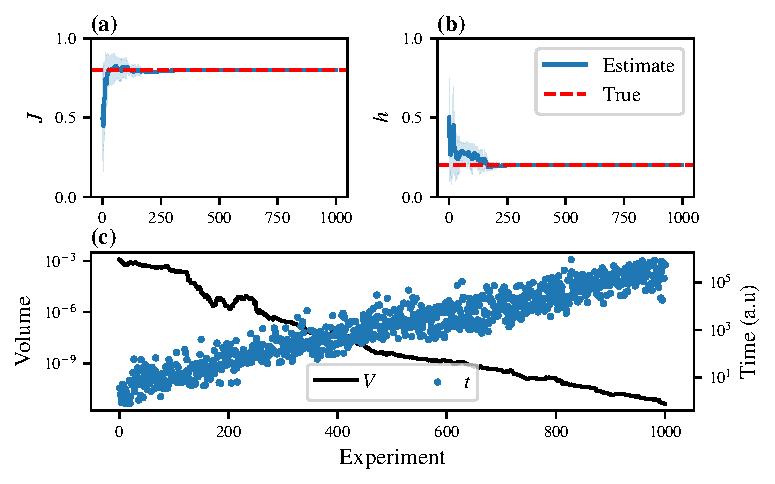
\includegraphics{theoretical_study/figures/standard_ising_qhl.pdf}
    \end{center}

    \caption[\Glsentrylong{qhl} for the standard Ising model]{
        \Acrlong{qhl} for the standard Ising model, where terms are grouped by their functionality, 
        as in \cref{eqn:ising_standard_form}. 
        \textbf{a-b,} the parameter estimates' progression against training \glspl{experiment}, 
            with the corresponding term labelling the $y$-axis. 
        The parameters are presented in arbitrary units of energy. 
        \textbf{c,} the \gls{volume} of the parameter distribution at each experiment, 
            as well as the evolution time chosen by the \gls{edh}. 
        \figtableref
    }
    \label{fig:ising_two_param_learning}
\end{figure}

\begin{figure}
    \begin{center}
        % \QMLAfig{Nov_18/13_56/fully_param_ising_qhl.pdf}
        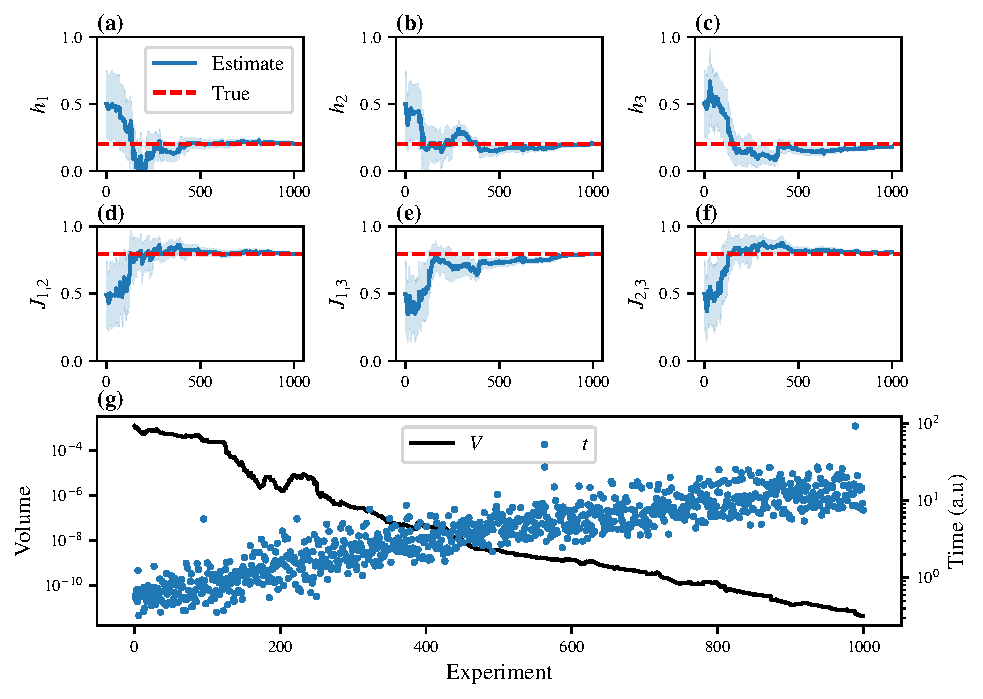
\includegraphics{theoretical_study/figures/fully_param_ising_qhl.pdf}
    \end{center}
    \caption[\Glsentrylong{qhl} for the fully parameterised Ising model]{
        \Acrlong{qhl} for the fully parameterised Ising model, 
            where every interaction between pairs of sites are assigned unique parameters, 
            as in \cref{eqn:ising_fully_parameterised}. 
        \textbf{a-f}, the parameter estimates' progression against training \glspl{experiment}, 
            with the corresponding term labelling the $y$-axis. 
            The parameters are presented in arbitrary units of energy. 
        \textbf{g,} the \gls{volume} of the parameter distribution at each experiment, 
            as well as the evolution time chosen by the \gls{edh}.  
        \figtableref
    }
    \label{fig:ising_fully_parameterised}
\end{figure}

\begin{figure}[t]
    \begin{center}
        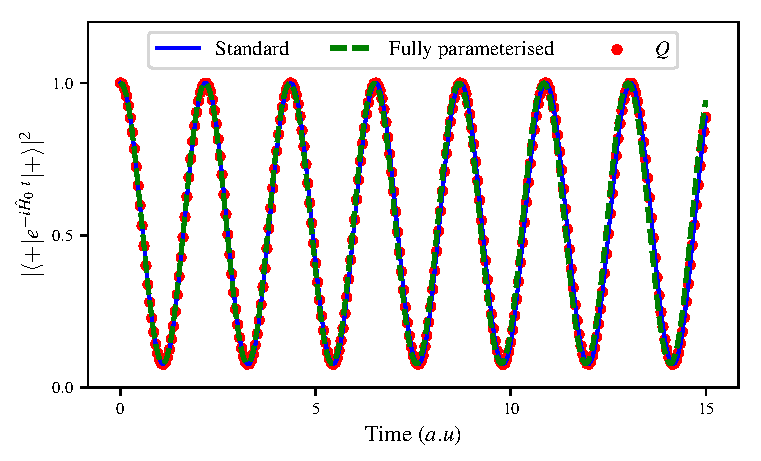
\includegraphics{theoretical_study/figures/dynamics.pdf}
    \end{center}
    \caption[Ising model forms' dynamics]{
        Dynamics reproduced by Ising models using the standard form (blue, training shown in \cref{fig:ising_two_param_learning}) 
        and the fully parameterised form (dotted green, training in \cref{fig:ising_fully_parameterised}), 
        compared with dynamics for the true system, \gls{q} (red dots).
        $\ho$ for $Q$ is given by the standard form, \cref{eqn:ising_standard_form}, with parameters set arbitrarily to $J=0.8$ and $h=0.2$.
        The \acrlong{bf} favours the standard formalism over the fully parameterised, with  a value of $\mathcal{B}=10^{19}$.
        \figtableref
    }
    \label{fig:ising_model_types_dynamics}
\end{figure}


We first construct models under each of these forms to verify \gls{qhl} is capable of learning in this regime:
    we train using the standard Ising model (\cref{eqn:ising_terms} as $\ho$ in \cref{fig:ising_two_param_learning}),
    and separately using the fully parameterised model (\cref{eqn:ising_fully_parameterised} as $\ho$ in \cref{fig:ising_fully_parameterised}).
Ultimately, these two cases give the same \gls{hamiltonian} when we set $J_{\bkl} = J; \ h_k = h \ \forall k,l$.
The fully parameterised model will learn the same parameters as the standard Ising model,
    and we can take the \gls{bf} between them to determine which parameterisation is favourable.
Encouragingly, both models learned the parameters to high precision, although neither model converged,
    i.e. the \gls{volume} continues to reduce exponentially in both cases.
This outcome is common: training is not guaranteed to converge\footnotemark, 
    so it can be impractical to seek saturation in the training phase for every model, 
    since this may require a very large number of \glspl{experiment} and \glspl{particle}. 
\footnotetext{When the model being trained is $\ho$, the volume may not saturate until numerical precision is reached.}
It would be preferable for each model's parameterisation to have converged before comparing them, 
    but in practice this is infeasible due to the indefinite resources required; 
    model comparisons must rely on limited training schedules which are presumed to reflect the overall ability of 
    the models to capture \gls{q}'s dynamics. 
We will see throughout this thesis\footnotemark \ that the choice of such training resources, namely \gls{nexp}, \gls{nprt}, 
    has a large impact on the outcome of \gls{qmla}, for example through misleading comparisons between models 
    in the case where the better model's training was under performant. 
This capacity for error is mitigated by combining many \glspl{instance} together in 
    a \gls{qmla} \gls{run}, such that any conclusions drawn rely on the average performance, 
    where strong models are likely to perform better overall, even given access to limited resources. 
\footnotetext{
    Including \cref{sec:family_classification} where we study the effect of varying resources on \gls{qmla}'s outcome
    in the context of lattice systems described here.
}
\par 

The dynamics produced by both models are shown in \cref{fig:ising_model_types_dynamics}:
    the dynamics are almost indistinguishable by eye, but the standard Ising model, 
    which in this case is $\ho$, outperforms the fully parameterised model, 
    by a \gls{bf} of $\mathcal{B} = 10^{19}$.
This serves as a good \emph{sanity check}, confirming our expectation that 
    the \gls{bf} will favour the simpler model (i.e. fewer parameters) even when both models 
    are trained to a high precision to very similar parmaeters, and are difficult to distinguish through human intuition. 


\section{Heisenberg model}\label{sec:heisenberg}
Generalising the Ising model, the Heisenberg \gls{hamiltonian} is another model for magnetic systems consisting of a set of 
    spins on a lattice \cite{greiner2012thermodynamics}. 
It builds on the Ising model by additionally considering the spins' rotations about the $x$- and $y$-axes, generally stated as 
\begin{equation}
    \label{eqn:heisenberg_model_general}
    \hat{H}_H(\cc) = 
    \sum\limits_{\bkl \in \cc} J^x_{kl} \  \s^x_k \s^x_l
    + \sum\limits_{\bkl \in \cc} J^y_{kl} \ \s^y_k \s^y_l
    + \sum\limits_{\bkl \in \cc} J^z_{kl} \ \s^z_k \s^z_l
    + \sum\limits_{k=1}^{N} h_k \s^z_k.
\end{equation}

We can consider a number of formulations of the Heisenberg model, by considering whether the interaction
    parameters are completely unique for each pair of spins in each axis, 
    or  are shared by pairs of spins.
We list a number of prominent representations within the family of Heisenberg models in \cref{table:heisenberg_models}. 
\begin{table}[H]
    \begin{center}
        \begin{tabular}{crrrr}
             & $J^{x}_{kl}$ & $J^{y}_{kl}$ & $J^{z}_{kl}$ & $h_{k}$ \\
            \hline
            XXX & $J^x$ & $J^x$ & $J^x$ & $h$ \\
            XXZ & $J^x$ & $J^x$ & $J^z$ & $h$ \\
            XYZ (standard) & $J^x$ & $J^y$ & $J^z$ & $h$ \\
            Fully parameterised & $J^x_{kl}$ & $J^y_{kl}$ & $J^z_{kl}$ & $h_k$ \\
            
        \end{tabular}
    \end{center}
    \caption[Forms of Heisenberg model]{
        Heisenberg model forms: varying whether the interaction parameters $J^{w}_{kl}$ are shared among pairs of spins
        give distinct descriptions, all of which are within the family of Heisenberg models. 
    }
    \label{table:heisenberg_models}
\end{table}

Again, there are a number of possibile models to test, 
    although we can reasonably expect these to follow the same arguments as for the Ising model cases: 
    increasing generality -- at the expense of larger parameter dimension -- 
    requires more resources to learn to a reasonable level.    
In \cref{chapter:ga} we will consider the fully parameterised model, 
    but here focus on the more restrictive Heisenberg-XYZ model:
    the parameters and terms of interest are then captured by \cref{eqn:heisenberg_terms}.

\begin{subequations}
    \begin{equation}
        \al_{H} = \irow{ J^x & J^y & J^z & h}    
    \end{equation}

    \begin{equation}
        \terms_{H} = \icol{
            \sum\limits_{\bkl \in \cc} \ \s^x_k \s^x_l \\
            \sum\limits_{\bkl \in \cc} \ \s^y_k \s^y_l \\
            \sum\limits_{\bkl \in \cc} \ \s^z_k \s^z_l \\
            \sum\limits_{k=1}^{N} \ \s^z_k  \\
        }.
    \end{equation}
    \label{eqn:heisenberg_terms}
\end{subequations}


\section{Hubbard model}\label{sec:hubbard}
Another representation of solid state matter systems is given by the Hubbard model 
    \cite{hubbard1963electron, scalettar2016introduction, hubbard2013}.
The Hubbard model deals with systems of correlated fermions, 
    allowing spins to \emph{hop} between sites and to localise on sites.
Spins are \emph{correlated} in this model because the spin on any site is subject to the Coulomb interaction, 
    i.e. a repulsive force due to the presence of another electron on the same site,
    so it is energetically favourable for spins to arrange across sites.
Note the Hubbard model is synonymous with the \gls{fh} model, 
    which can be used to distinguish the statistics from a set of fermions from the statistics of a similar set of bosons, given by the Bose-Hubbard model.
In this thesis we will not study the Bose-Hubbard model, but will use the subscript FH to distinguish the (Fermi-)Hubbard model from the Heisenberg model 
    $\hat{H}_{H}$, \cref{eqn:heisenberg_model_general}.
The Hubbard model is generally stated in second quantisation as

\begin{equation}
    \label{eqn:hubbard}
    \hat{H}_{FH}(\cc) = 
    - \sum_{s \in \{\uparrow, \downarrow\}} \sum_{ \bkl \in \mathcal{C}} t^{s}_{\bkl} \left( \hat{c}^{\dagger}_{ks} c_{ls} + \hat{c}^{\dagger}_{ls} c_{ks} \right) 
    + \sum_{k}^{N} U_k \hat{n}{k\uparrow}\hat{n}_{k\downarrow} 
    + \sum_{k}^{N} \mu_k \left( \hat{n}_{k\uparrow} + \hat{n}_{k\downarrow} \right)     
\end{equation}
    where 
\begin{easylist}[itemize]
    & $\hat{c}_{ks}$ and $\hat{c}^{\dagger}_{ks}$ are respecitvely the fermionic annihilation and creation operators for spin $s \in \{ \uparrow, \downarrow \}$ on site $k$;
    & $\hat{n}_{ks} = \hat{c}^{\dagger}_{ks} \hat{c}_{ks}$ is the onsite term, i.e. a counting operator to count the number of spins $s$ on site $k$;
    & $t^s_{\bkl}$ is the kinetic (hopping) term for spin $s$ between sites $k$ and $l$; 
    & $U_k$ is the onsite (repulsion) energy for site $k$;
    & $\mu_k$ is the chemical potential for $k$;
    & $N$ is the number of sites in the system.
\end{easylist}
\par

Again, we can achieve differing physics by controlling whether the parameters are shared (e.g. $t_{\bkl}^s$), 
    with similar consequences to the Ising and Heisenberg models, where additional parameterisation
    comes at the expense of slower/worse performance in training. 
We list a subset of possible configurations in \cref{table:hubbard_model_types}, 
    again here we will use the standard form for the remainder of this chapter, \cref{eqn:hubbard_terms}. 

\begin{table}[H]
    \begin{center}
        \begin{tabular}{crrrr}
                & $t^{\uparrow}_{\bkl}$& $t^{\downarrow}_{\bkl}$ & $U_k$ & $\mu_k$ \\
            \hline 
            Standard & $t$ & $t$ & $U$ & $\mu$ \\
            Fully parameterised & $t^{\uparrow}_{\bkl}$  & $t^{\downarrow}_{\bkl}$&  $U_k$ & $\mu_k$ \\
        \end{tabular}
    \end{center}
    \caption[Forms of Hubbard model]{
        Forms of Hubbard model. Varying whether parameters $t^{s}_{\bkl}, U_k, \mu_k$ are shared 
        across sites gives distinct models.
    }
    \label{table:hubbard_model_types}
\end{table}
    

\begin{subequations}
    \begin{equation}
        \al_{FH} = \irow{ t^{\uparrow} & t^{\downarrow} & U & \mu}
    \end{equation}
    
    \begin{equation}
        \terms_{FH} = \icol{ 
            \sum\limits_{ \bkl \in \cc }
                ( 
                    \hat{c}^{\dagger}_{k,\uparrow} \hat{c}_{l,\uparrow} + \hat{c}^{\dagger}_{l,\uparrow} \hat{c}_{k,\uparrow} 
                ) \\
            \sum\limits_{ \bkl \in \cc }
                ( 
                    \hat{c}^{\dagger}_{k,\downarrow} \hat{c}_{l,\downarrow} + \hat{c}^{\dagger}_{l,\downarrow} \hat{c}_{k,\downarrow} 
                ) \\
            \sum\limits_{k=1}^{N} \hat{n}_{k\uparrow} \hat{n}_{k\downarrow} \\
            \sum\limits_{k=1}^{N} \bk{\hat{n}_{k\uparrow}  + \hat{n}_{k\downarrow} }
        }.
    \end{equation}
    
    \label{eqn:hubbard_terms}
\end{subequations}


\subsection{Jordan Wigner transformation}\label{sec:jordan_wigner}
In order that the Hubbard model is simulateable with qubits\footnotemark, 
    it must first undergo a mapping from the fermionic 
    representation to a spin system representation; 
    such a mapping is given by the \gls{jwt} \cite{jordan1993paulische, steudtner2018fermion}.
We implement the \gls{jwt} within \gls{qmla} through \ttt{OpenFermion}'s \ttt{fermilib} package \cite{mcclean2020openfermion}.
\footnotetext{Or simulations of qubits, as in this thesis.}
\par 

In second quantisation, 
    the fermions on the lattice can occupy one (or a superposition of) \emph{modes}, 
    for example, spin $\uparrow$ on the site indexed $3$ is a mode. 
The system can then be given by a state in the \emph{number basis}, 
\begin{equation}
    \ket{\psi_f} = \ket{ n_{m_1}, n_{m_2}, \dots , n_{m_n} },
\end{equation}
where $n_{m_i}$ is the number of fermions on mode $m_i$ and there are $n$ modes in total.

$\hat{c}^{\dagger}_{m_i}$ \ ($\hat{c}_{m_i}$) is the creation (annihilation) operator
    on the mode $m_i$: it acts on the system by adding (removing) a fermion to (from) $m_i$:
\begin{subequations}
    \begin{equation}
        \hat{c}^{\dagger}_{m_i} \ket{\psi_f} = \ket{ n_{m_1}, \dots , n_{m_i}  + 1,  \dots , n_{m_n} }, 
    \end{equation}
    \begin{equation}
        \hat{c}_{m_i} \ket{\psi_f} = \ket{ n_{m_1}, \dots , n_{m_i} - 1,  \dots , n_{m_n} }.
    \end{equation}            
\end{subequations}

In the Hubbard model, we assign a mode for each combination of spin $s \in \{\uparrow, \downarrow\}$
    with each site $k$, i.e. the system is in the state
\begin{equation}
    \label{eqn:hubbard_number_state}
    \ket{\psi_{FH}} = \ket{ n_{1\uparrow}, n_{1\downarrow}, \dots , n_{N\uparrow}, n_{N\downarrow} }.
\end{equation}
\par 

In particular, since fermions obey the Pauli exclusion principle, 
    i.e. every spin/site can be occupied by at most one electron, and we can view them as two-level systems, 
    so we have $n_{sk} \in \{0, 1\} \forall s, k$,     
We therefore use a similar system to the number basis: 
    a qubit registered as $\ket{0}$ corresponds to an empty mode, while $\ket{1}$ holds a fermion. 
Empty lattices are thus given by $\ket{0}^{\otimes 2N}$. 
Then, in analogue with the annihilation and creation operators, we introduce operators $\s^{+}, \s^{-}$ such that 
\begin{subequations}
    \begin{equation}
        \s^{+} = \begin{pmatrix}
            0 & 0 \\ 1 & 0 
        \end{pmatrix}
        \Longrightarrow \s^{+} \ket{0} = \ket{1}
    \end{equation}

    \begin{equation}
        \s^{-} = \begin{pmatrix}
            0 & 1 \\ 0 & 0 
        \end{pmatrix}
        \Longrightarrow \s^{-} \ket{1} = \ket{0}
    \end{equation}
\end{subequations}
   

Then, to map the number basis of \cref{eqn:hubbard_number_state} to a state which can be prepared on qubits, 
    the \gls{jwt} assigns a single qubit to each mode, 
    where qubits are ordered simply by the site index and spin type, 
    as shown in \cref{table:jordan_wigner_indices}. 
The \gls{jwt} can be summarised by mapping -- for the mode $m$ -- the creation (annihilation) operator
    $\hat{c}^{\dagger}_{m}$ \ ($\hat{c}_{m}$), to an operator which adds (removes) a spin to (from) the corresponding state 
    through the operator $\s_{m}^{+}$ \ ($\s_{m}^{-}$). 

\begin{subequations}
    \label{eqn:jordan_wigner}
    \begin{equation}
        \hat{c}_{m} \rightarrow (\s^z)^{\otimes k-1} \otimes \s^{-} \otimes (\s^z)^{\otimes 2N-1}
    \end{equation}
    \begin{equation}
        \hat{c}_{m}^{\dagger} \rightarrow (\s^z)^{\otimes k-1} \otimes \s^{+} \otimes (\s^z)^{\otimes 2N-1}
    \end{equation}
\end{subequations}

% Note the \gls{jwt} acts on all modes/qubits other than the target with $\s^z$, since 
For example, an empty 2-site lattice $\ket{\psi_0}$ is acted on by a creation operator on mode $3$, corresponding to spin $\uparrow$ on site $2$:
\begin{equation}
    \hat{c}^{\dagger}_{2\uparrow} \ket{0000}  = \hat{c}^{\dagger}_{3} \ket{0000} = \s^z_1 \s^z_2 \s^{+}_3 \s^z_4 \ket{0000} = \ket{0010}. 
\end{equation}

\begin{table}
    \begin{center}
        \begin{tabular}{cccc}
            Mode & Site & Spin & Qubit \\
            \hline
            $1$ & $1$ & $\uparrow$ & $1$ \\
            $2$ & $1$ & $\downarrow$ & $2$ \\
            $3$ & $2$ & $\uparrow$ & $3$ \\
            $4$ & $2$ & $\downarrow$ & $4$ \\
             & \vdots &  & \\
            $2N -1$ & $N$ & $\uparrow$ & $2N-1$ \\
            $2N$ & $N$ & $\downarrow$ & $2N$ \\
        \end{tabular}
    \end{center}
    \caption[Jordan Wigner mode/qubit indices]{Jordan Wigner mode/qubit indices.}
    \label{table:jordan_wigner_indices}
\end{table}


\subsection{Half filled basis}
In principle there can be $2N$ spins on a lattice of $N$ sites, 
    although in general we will restrict to the case where there are $N$ spins in the lattice, 
    known as \emph{half-filling}, such that \cref{eqn:hubbard_number_state} is effectively projected into the subspace 
    spanned by half-filled basis states. 
For example, with $N=2$
\begin{equation}
    \label{eqn:hubbard_half_filled_basis_states}
    \{
        \ket{ 1100 }, \ket{ 1010 }, \ket{ 1001 }, 
        \ket{ 0101 }, \ket{ 0110 }, \ket{ 0011 }
    \}
\end{equation}

Therefore, in the design of probes for training Hubbard models, 
    we can generate probes in the subspace spanned by half-filled states. 

\section{Model learning for lattices}
Finally, then, we can use the lattice systems introduced in \cref{sec:lattices,sec:ising,sec:heisenberg,sec:hubbard}
    as first case studies for \gls{qmla}. 
Each $\cc \in \mathbb{C}$ can specify a unique model under their standard forms:
    \cref{eqn:ising_terms} for Ising, \cref{eqn:heisenberg_terms} for Heisenberg 
    and \cref{eqn:hubbard_terms} for Hubbard models.     
We can then devise a simple \gls{es} which only tests the models corresponding to lattices in $\mathbb{C}$, 
    with no further model generation, i.e. \cref{alg:lattice_exploration_strategy}, 
    and compares every pair of models through \glspl{bf}, 
    deeming the champion as that which wins the largest number of comparisons, 
    as in \cref{alg:lattice_exploration_strategy_consolidation}.

\begin{algorithm}
    \caption{Lattice exploration strategy: model generation}
    \label{alg:lattice_exploration_strategy}
    \DontPrintSemicolon
    \KwIn{ $\mathbb{C}$ \tcp*[1]{Set of lattice configurations}}

    \KwOut{$\{ \hi \}$ \tcp*[1]{Set of models to tests}}\;

    $\mathbb{H}$ = \{ \}\;
    \For{$\cc \in \mathbb{C}$}{
        $\hi \gets$ \ttt{map\_lattice\_to\_model}($\cc$)\;
        $\mathbb{H} \gets \mathbb{H} \cup \{ \hi\}$
    }
    return $\mathbb{H}$
\end{algorithm}

\begin{algorithm}
    \caption{Lattice exploration strategy: consolidation}
    \label{alg:lattice_exploration_strategy_consolidation}
    \DontPrintSemicolon
    \KwIn{ $\mathbb{H}$ \tcp*[1]{Set of trained models}}

    \KwOut{$\hp$ \tcp*[1]{Favoured model}}\;

    \For{ $\hi \in \mathbb{H}$}{
        $s_i \gets 0 $ \tcp*[1]{Score for every model}
    }

    \For{$\hi \in \mathbb{H}$}{
        \For{$\hj \in \mathbb{H}\setminus \{\hi\}$}{
            $\bij \gets BF(\hi, \hj)$ \tcp*[1]{Compute Bayes factor via \cref{alg:bayes_factor}}

            \If{$\bij > 1$}{
                $s_i \gets s_i + 1$ \tcp*[1]{$\hi$'s score increases if it is the stronger model}
            }
        }
    }
    $\hp \gets \argmax\limits_{s_i} \bk{\hi}$

    return $\hp$
\end{algorithm}


\begin{figure}
    % \QMLAfig{Nov_19/12_04/lattice_qmla_summary.pdf}
    \begin{center}
        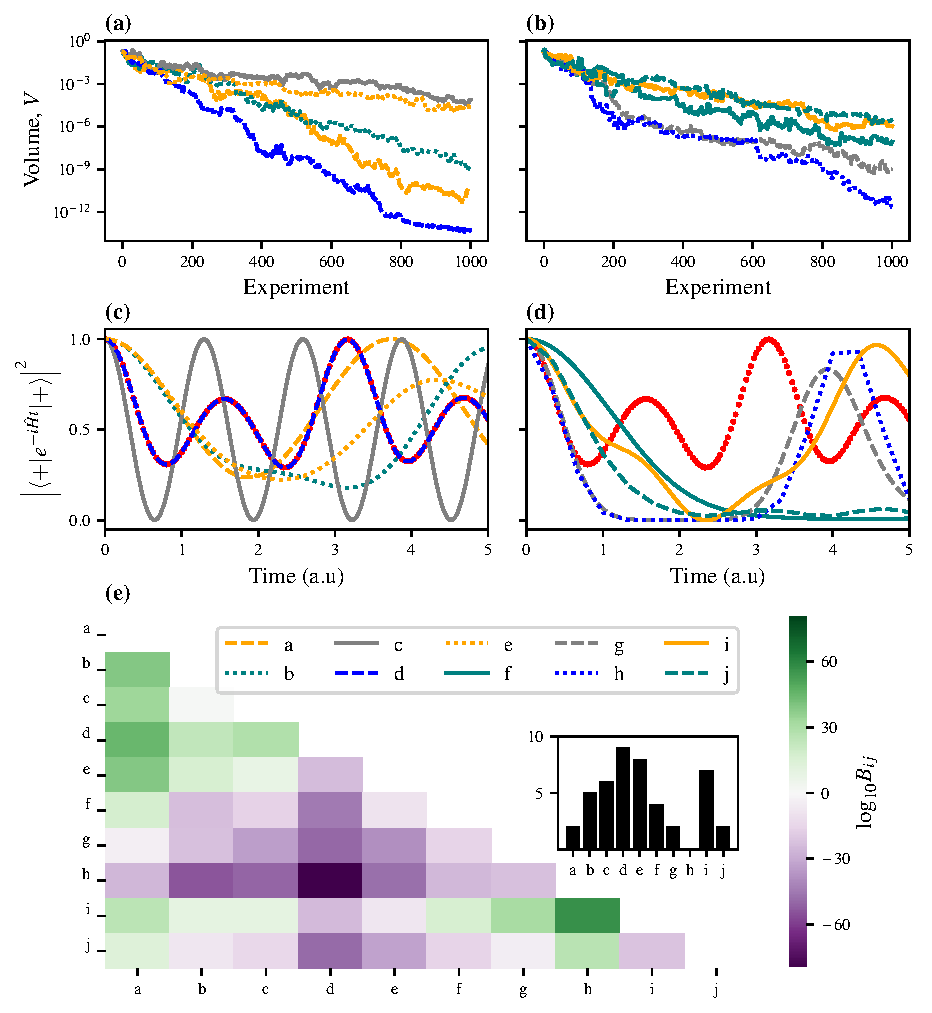
\includegraphics{theoretical_study/figures/lattice_qmla_summary.pdf}
    \end{center}
    \caption[QMLA for prescribed set of lattices under Ising formalism]{
        \gls{qmla} for prescribed set of lattices under Ising formalism. 
        The lattice indices correspond to those in \cref{fig:lattices}, 
            and the true system is given by lattice $d$. 
        \textbf{a-b,} the decrease in \gls{volume} for each model's training phase (spread over two plots for readibility).
        \textbf{c-d,} trained models are used to reproduce dynamics, compared with the dynamics of the
            true system (red dots). 
        \textbf{e,} Heatmap of $\log_{10} \bij$ between every pair of models. The \gls{bf} is read as 
        $i$ versus $j$, where $i$ is the model on the $y$-axis and $j$ is the model on the $x$-axis. 
        $\log_{10} \bij > 0$ (green) favours the model listed on the $y$-axis;
        $\log_{10} \bij < 0$ (purple) favours the model listed on the $x$-axis.
        The inset shows the number of \gls{bf} comparisons won by each model, i.e. the models' scores. 
        \figtableref
    }
    \label{fig:lattice_qmla_eg}
\end{figure}    

For example, we adopt the fully connected four site lattice ($d$ in \cref{fig:lattices})
    as the true lattice specifying $\ho$, under the Ising formalism (\cref{eqn:ising_model_full}).
We run \gls{qmla} by training the ten models corresponding to the ten lattices,  \cref{fig:lattice_qmla_eg}\textbf{a-b};
    comparing the models predictive power, \cref{fig:lattice_qmla_eg}\textbf{c-d},
    through \gls{bf} (\cref{fig:lattice_qmla_eg}\textbf{e}), 
    and choosing the model which wins the largest number of \gls{bf} contests. 
In this example, $\ho$ is stronger than every alternative model according to the \glspl{bf}, 
    and is hence determined as $\hp$. 

\section{Complete QMLA run for lattice sets}
In order to test \gls{qmla} robustly, 
    we can use each of the lattices shown in \cref{fig:lattices} to specify $\ho$, 
    to ensure the algorithm is capable of finding the underlying model of arbitrary complexity, 
    within the constraints of a prescribed model set\footnotemark. 
\footnotetext{The remainder of this thesis is dedicated to cases where we do not prescribe the model set, but instead generate models dynamically.}
Moreover, we can extend this test to the Heisenberg and Hubbard formalisms; 
    note that due to the overhead given by the \gls{jwt} (\cref{sec:jordan_wigner}), i.e. the requirement of two qubits per site, 
    we restrict study of the Hubbard model to lattices $a-e$ for practicality\footnotemark.
\footnotetext{
    The limitation of Hubbard models to $3$-site lattices is due to the $6$-qubit models required via the \gls{jwt}.
    The primary expense of simulation is the complete unitary evolution, 
        requiring calculation of $e^{-i \hi t}$ for each particle's likelihood calculation at every training experiment. 
    Training becomes infeasible for systems requiring $\gtrapprox9$ qubits, whereas moving to $5$-site lattices would require $10$-qubit models.
    We include a mixture of lattices up to $4$ sites for the Hubbard model, and some further models up to $6$ sites for the Ising and Heisenberg models.
}
By running 10 independent \gls{qmla} \glspl{instance} for each lattice under each formalism,
    we can gauge the success rate of the algorithm for distinguishing basic lattices from each other. 
We present the result of these tests in \cref{fig:lattice_success_rates},   
    finding in all cases that \gls{qmla} identifies $\ho$ with success rates at least $70\%$. 
A general trend appears to emerge -- especially in the case of the Hubbard model --
    where target models of higher dimension are identified less often. 
This can likely be attributed to the training resources provided:
    here models are trained with $\Ne=1000 \Np=4000$, 
    which are clearly sufficient for training models of few qubits/parameters, 
    but may not allow larger models to train well.  
In the next section we investigate whether increasing \gls{nexp}, \gls{nprt} leads to higher success rates in general, 
    and find a strong correlation between training resources and \gls{qmla} success rate. 
We therefore expect that the results for large target models could be improved by drastically increasing the training resources, 
    although for practicality, we do not perform such a test.

\par 

\begin{figure}
    \begin{center}
        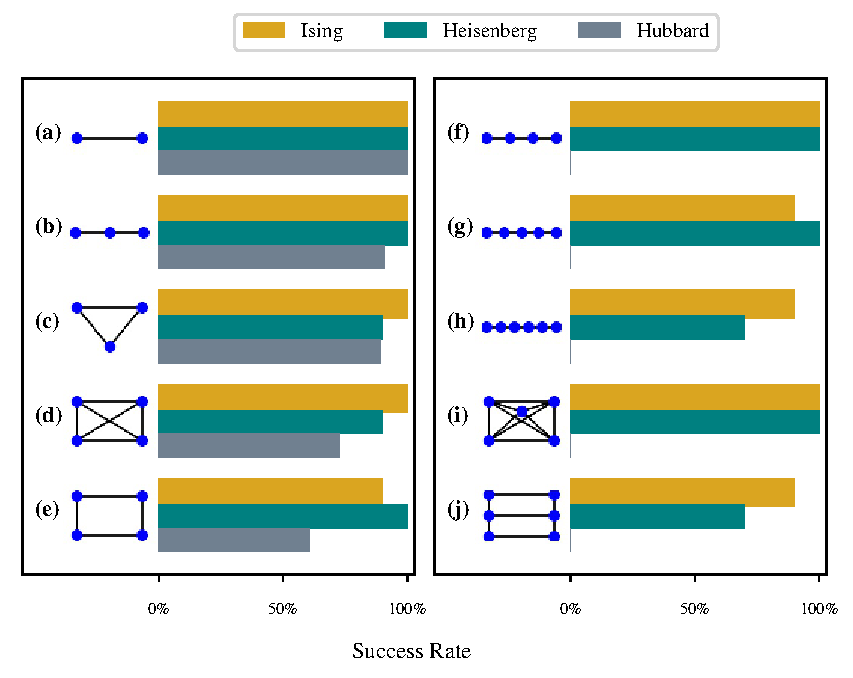
\includegraphics{theoretical_study/figures/lattice_successes_two_column.pdf}
    \end{center}
    \caption[QMLA success rates for lattices]{
        Rates of success for \gls{qmla} under various conditions. 
        Each lattice is set as the \gls{true model} $\ho$ for ten independent instances. 
        In each instance, the \gls{es} considers the available lattices 
            (\textbf{a-j} for Ising and Heisenberg cases and \textbf{a-e} for the Hubbard case), 
            and selects a \gls{champion model} $\hp$ as that most consistent with data generated by $\ho$. 
        The figure displays the rate at which each lattice is correctly identified as $\ho$
            under standard Ising, Heisenberg and Hubbard formalisms. 
        \figtableref
    }
    \label{fig:lattice_success_rates}
\end{figure}    


While there is compelling evidence that \glspl{bf} can be used for model selection in general \cite{berger1996intrinsic}, 
    this straightforward test verifies that the \gls{bf} is a fair mechanism by which to distinguish between 
    models in the context of candidate descriptions for quantum systems. 
In general it will not be possible to prescribe the set of models to test, 
    although this might serve as a straightforward mechanism for the calibration of quantum devices.
Suspected miscalibrations can be used in the design of such a set of models, 
    along with a target $\ho$ which the device should be able to implement. 
By testing such a prescribed set and determining $\hp$, 
    we can map the miscalibration between the intended and actual operations. 
In the ideal case, where it is mostly believed the device works, 
    this application of \gls{qmla} may allow for fast, automated \emph{verification} of the device:
    if \gls{qmla} finds $\hp=\ho$ with high success given reasonable opportunity to miscompute, 
    it may be sufficient verification that the device behaves as desired, 
    or at least part thereof. 

\section{Model family classification}\label{sec:family_classification}
\begin{figure}[t]
    \begin{center}
        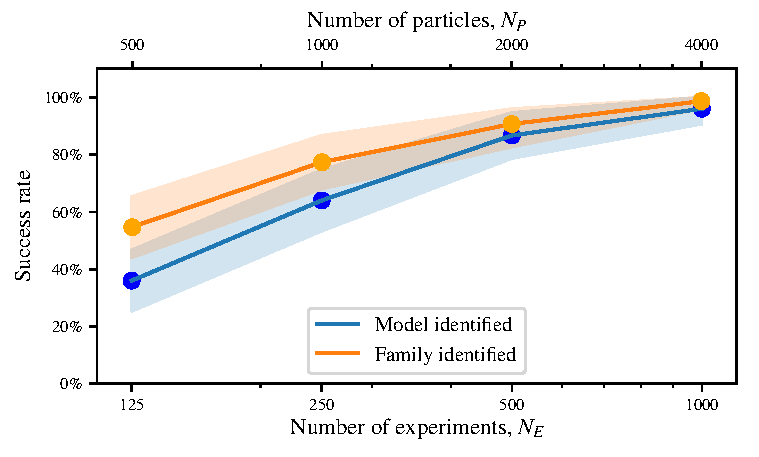
\includegraphics{theoretical_study/figures/model_family_search.pdf}
    \end{center}
    \caption[QMLA outcomes for varying training resources]{
        \gls{qmla} outcomes for varying training resources. 
        Independent \glspl{es} are implemented for Ising, Heisenberg and Hubbard families, 
            with $\ho$ cycling through lattices (a-f) for the Ising and Heisenberg cases, 
            and (a-c) for the Hubbard case, where lattices' connectivity are as depicted in \cref{fig:lattices}.
        Each latttice in each famility is tested as $\ho$ in five \glspl{instance}, so there are 75 \glspl{instance} per datapoint. 
        The success rates are shown for \gls{qmla} identifiyng the correct model precisely (blue),
            as well as classifying the correct model family (orange), 
            against the numbers of \glspl{experiment} and \glspl{particle} used to train each candidate model. 
        \figtableref
    }
    \label{fig:family_classification}
\end{figure}



\glsreset{es}
\glsreset{et}
Recall from \cref{sec:qmla_protocol} (and \cref{fig:qmla_overview}\textbf{(e)}) that \gls{qmla} 
    can grow multiple \glspl{et} concurrently, each corresponding to a unique \gls{es}. 
This functionality permits \glspl{et} of different underlying physical assumptions, 
    and can therefore be used to examine alternative formalisms in parallel.
For instance, in order to examine the target system, \gls{q}, 
    we can independently run \glspl{es} for each of the Ising, Heisenberg and Hubbard model \emph{families}:
    \gls{qmla} first deems the most appropriate model under each formalism, $\hp_S$,
    before consolidating $\{\hp_S\}$ and declaring the global \gls{champion model}, $\hp$. 
$\hp$ therefore encodes which family best describes the system of interest, \gls{q}:
    even if the precise model is not found, $\hp \neq \ho$, we can still classify the 
    model family -- i.e. the underlying physical mechanism -- which is most useful for describing \gls{q}. 
\par 

Earlier in this chapter, we alluded to a fundamental question in the discussion of model training and comparison 
    through Bayesian inference, as underlies \gls{qhl}:
    to what extent is a trained model undermined by its \emph{limited} training resources\footnotemark, 
    and what resources should be granted in order to retrieve reliable outcomes?
As usual in \gls{ml} methods, this represents a trade-off between the results of the algorithm 
    against training time and computational resources required.
\footnotetext{
    Recall the main resources for model training: the number of \glspl{experiment} performed, \gls{nexp}, and the number of \glspl{particle} used during \gls{qhl}, \gls{nprt}.
}
\par

We combine the task of family classification 
    with non-exhaustive testing of the tradeoff between resources and outcomes.
In this case, we vary the target model $\ho$ as deriving again from the lattices in 
    \cref{fig:lattices}, 
    however we reduce the number of tested models in each case. 
\glspl{es} corresponding to the Ising and Heisenberg model consider lattices (a-f), 
    while the \gls{es} for the Hubbard model only consider (a-c). 
\cref{fig:family_classification} shows the rate at which the precise $\ho$ is identified, 
    as well as the rate with which family of $\ho$ is classified, 
    compared with increasing resources, \gls{nexp} and \gls{nprt}. 
As expected, a clear trend demonstrates that the success rates scale with resources,
    which we can leverage in practice in two core ways.
Firstly, we can simply ensure that the training regime for models is sufficiently robust, 
    such that we can reasonably expect models to have trained well, and therefore model comparisons can be trusted.
If \gls{qmla} does not give clear results, then, we may expect a clearer outcome from increasing \gls{nexp}, \gls{nprt}.
Secondly, we can mitigate the unpredictable\footnotemark failures of \gls{qmla} by running many \glspl{instance} per \gls{run}:
    one (or few \glspl{instance}) in a scarce-resource training regime are prone to error, 
    so in cases where we are unsure whether the resources provided are sufficient, 
    we must run enough independent \glspl{instance} to overcome these artefacts. 
\footnotetext{
    \gls{qmla} depends on several probabilistic processes which can cause misleading outcomes; 
    these are highlighted in \cref{sec:usage}. 
}
\par 

\gls{qmla}'s capacity to classify the family of model to which \gls{q} belongs suggests powerful 
    future applications of the framework, namely to automatically discover the type of physics underlying 
    systems of interest.
For example, \gls{qmla} could be used to classify whether a sample is ferromagnetic or antiferromagnetic;
    or further, is best described as a system of bosons or fermions.
